\subsection{Controller}
This subsystem will be in charge of handling requests to the endpoints of the services we will be utilizing in Synthify (YouTube, Spotify, Soundcloud, etc.)

\begin{figure}[h!]
	\centering
 	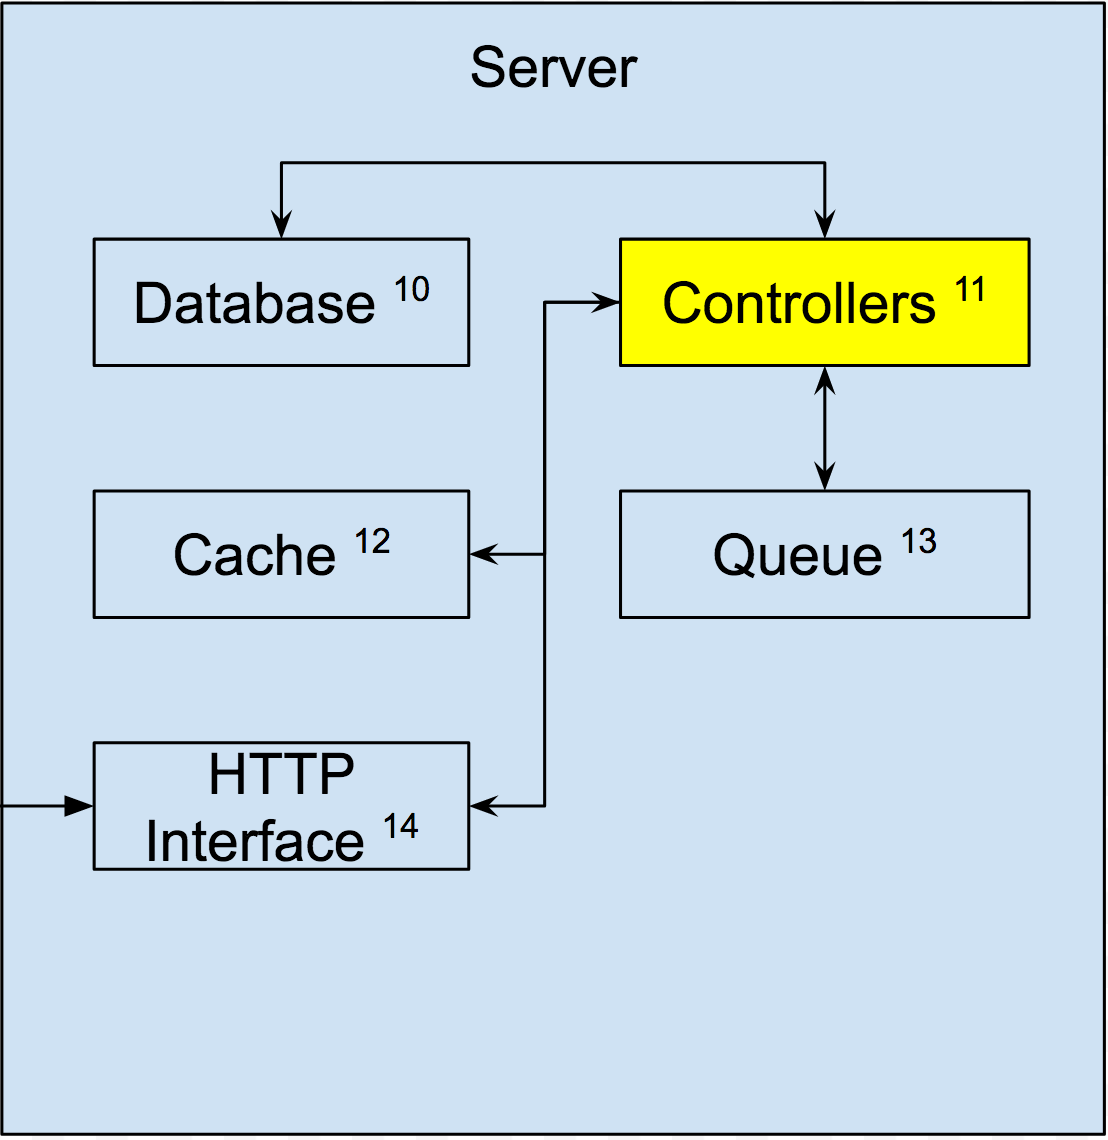
\includegraphics[width=0.60\textwidth]{images/server/server_controller.png}
 	\caption{Controller subsystem}
\end{figure}

\subsubsection{Assumptions}
N/A

\subsubsection{Responsibilities}
Responsibilities include setting up the proper endpoints with the correct HTTP requests (GET, POST, etc.) to other subsystems. The controller will directly interact with the database, queue, cache, and HTTP Interface subsystems.

\subsubsection{Subsystem Interfaces}
\begin {table}[H]
\caption {Cache interfaces} 
\begin{center}
    \begin{tabular}{ | p{1cm} | p{6cm} | p{6cm} | p{6cm} |}
    \hline
    ID & Description & Inputs & Outputs \\ \hline
    \#01 & Get user playlists & \pbox{6cm}{Connect spotify account} & \pbox{6cm}{User's playlists are retrieved}  \\ \hline
    \#02 & Get user info & \pbox{3cm}{N/A} & \pbox{3cm}{N/A}  \\ \hline
    \end{tabular}
\end{center}
\end{table}

\newpage
